\documentclass{beamer}
\usetheme{Marburg}

\usepackage[ansinew]{inputenc}
\usepackage[ngerman]{babel}
\usepackage{xcolor}
\usepackage{fancybox}


\usepackage{graphicx}
\usepackage{icomma,units}
\usepackage{amsfonts,amsmath,amssymb}
\usepackage{enumerate}
\usepackage{booktabs}
\usepackage{colortbl}


%Einstellung aus dem Pr�sentationstemplate
\beamersetuncovermixins{\opaqueness<1>{25}}{\opaqueness<2->{15}}

%Farbdefinitionen
\definecolor{dunkelgrau.80}{gray}{0.20}
\definecolor{dunkelgrau.60}{gray}{0.40}
\definecolor{hellgrau}{rgb}{0.95,0.95,0.95}
\definecolor{Dschungelgr\"{u}n}{cmyk}{0.99,0,0.52,0.2}
\definecolor{midblue}{rgb}{0.173,0.212,0.597}



\begin{document}

\title{Upper Rhine Region -- Oberrhein / Rhin Sup\'{e}rieur}   
\author{Pascal Bernhard} 
\date{\today}
\titlegraphic{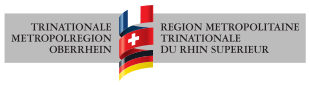
\includegraphics[width=3.8cm,height=0.9cm]{Logo_Trinationale_Metropolregion_Oberrhein.png}}
\logo{\includegraphics[scale=0.14]{logo-SF}}

%%%-------------------------------------------------------------------------------------------------------------------%%%

\begin{frame}
\titlepage
\end{frame}

%%%-------------------------------------------------------------------------------------------------------------------%%%

\begin{frame}
\frametitle{Table of Contents}\tableofcontents
\end{frame}

%%%-------------------------------------------------------------------------------------------------------------------%%%

\section{Geography} 

%%%

\begin{frame}\frametitle{Upper Rhine Region In Europe} 

\begin{center}
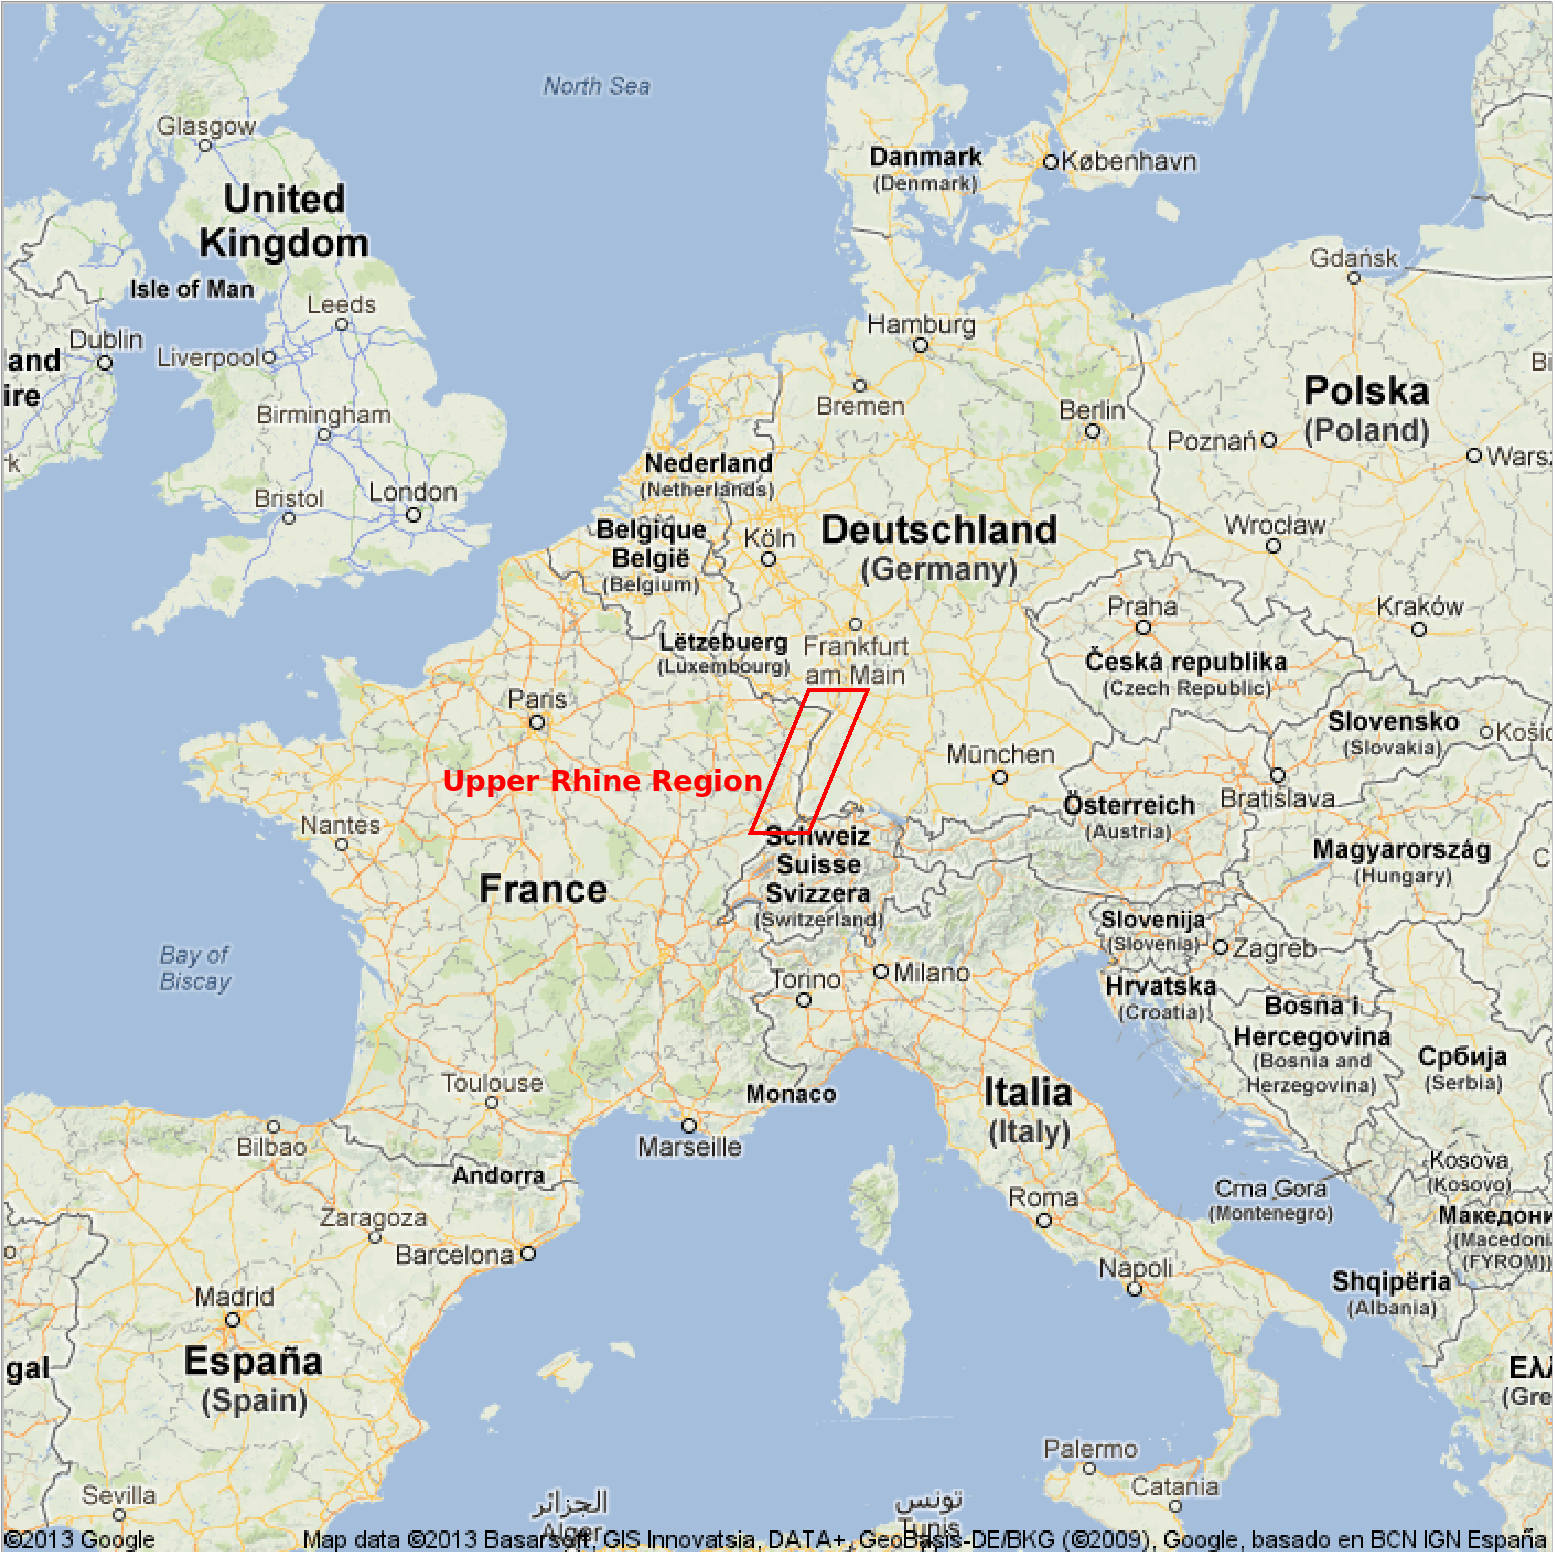
\includegraphics[width=7.03cm,height=7.0cm]{GoogleMaps_Western-Central-Europe.png} 
\end{center}

\end{frame}


%%%-------------------------------------------------------------------------------------------------------------------%%%

\begin{frame}\frametitle{Part of Europe's Main Economic Axis} 

\begin{center}
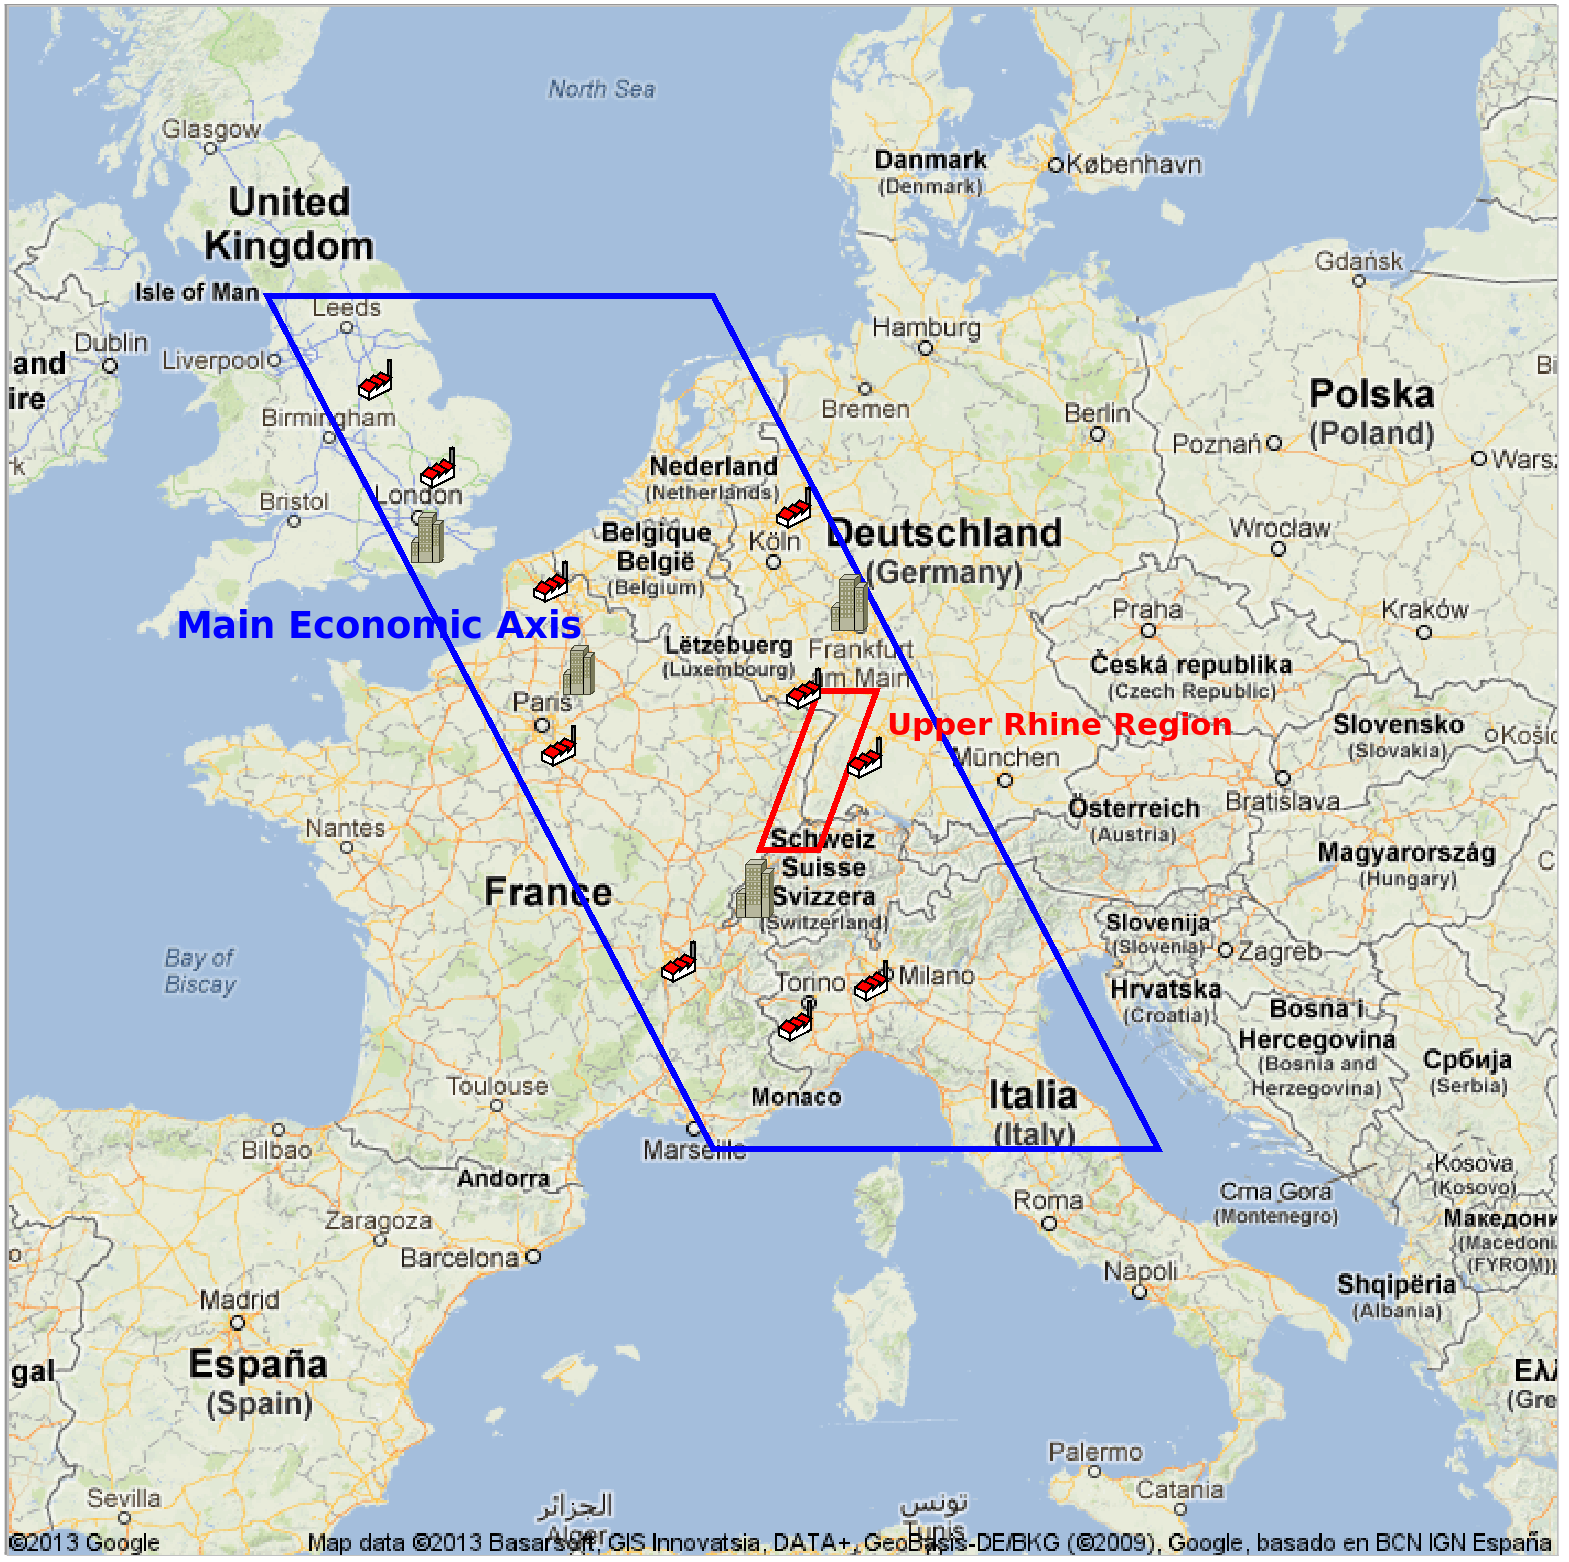
\includegraphics[width=7.03cm,height=7.0cm]{GoogleMaps_Western-Central-Europe_Parallelogramm_Pixbuff.png} 
\end{center}

\end{frame}


%%%-------------------------------------------------------------------------------------------------------------------%%%


\begin{frame}\frametitle{Topography} 

\begin{center}
\includegraphics[width=5.53cm,height=8.0cm]{Oberrheinkonferenz_Mandatsgebiet.png} 
\end{center}

\end{frame}

%%%-------------------------------------------------------------------------------------------------------------------%%%


\begin{frame}\frametitle{Geographic Features}


  \begin{itemize}
    \item Part of Europe's main economic axis\\
	 $\Rightarrow$ North-South Transport--Corridor (\textsl{Rotterdam-Genoa})\\
	 $\Rightarrow$ Need for transportation infrastructure

    \pause

    \item Rhine river as border and water way

    \pause

    \item Vosges mountains and Black Forest as touristic attraction along with Strasbourg \& Freiburg

    \pause

    \item Decentralized population structure with high population density\\
 	 $\Rightarrow$ No big metropolitan cities
   \end{itemize}

\end{frame}



%%%-------------------------------------------------------------------------------------------------------------------%%%

\section{Cooperation Among France, Switzerland \& Germany} 

\subsection{Common Issues}

\begin{frame}\frametitle{Policy Areas}

  \begin{itemize}
    \item Environmental problems
      \begin{enumerate}
	\item Air pollution
	\item Management of the Rhine river
      \end{enumerate}

      \pause

    \item Science \& Education\\
 	 $\Rightarrow$ Promotion of bilingualism (French-German)
  \end{itemize} 

\end{frame}

%%%-------------------------------------------------------------------------------------------------------------------%%%

\begin{frame}\frametitle{Policy Fields}

  \begin{itemize}
    \item Infrastructure
      \begin{enumerate}
	\item Transport infrastructure (\textsl{Transeuropean Networks})
	\item Integrating public transport systems across-borders
      \end{enumerate}

      \pause

    \item Economic Development
      \begin{enumerate}
	\item Marketing "`Upper Rhine"' as a brand
	\item Promotion of renewable energy
	\item Closer cooperation in vocational training
      \end{enumerate}
  \end{itemize} 

\end{frame}


%%%-------------------------------------------------------------------------------------------------------------------%%%


\begin{frame}\frametitle{Upper Rhine Conference} 

\begin{center}
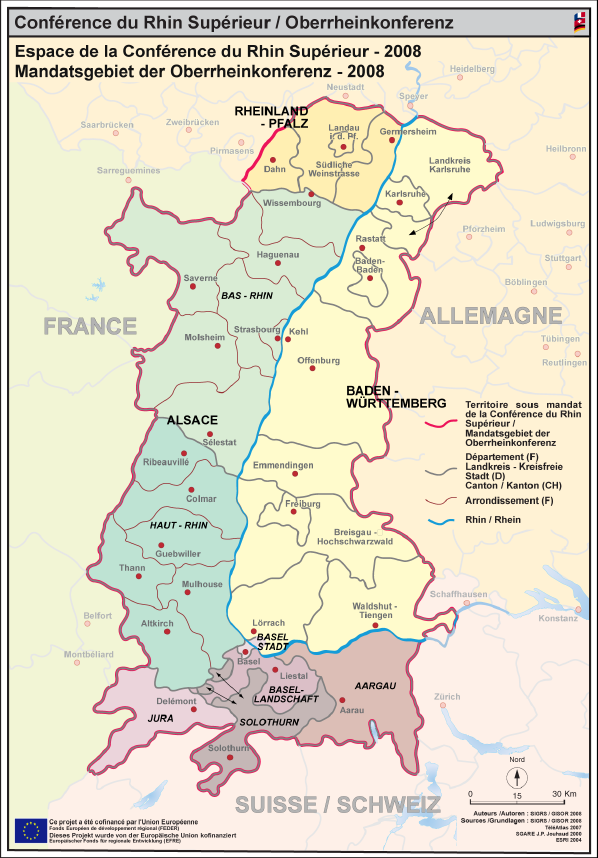
\includegraphics[width=5.53cm,height=8.0cm]{Mandatsgebiet_Oberrheinkonferenz.png} 
\end{center}

\end{frame}


%%%-------------------------------------------------------------------------------------------------------------------%%%
\section{Regional Institutions} 

\subsection{Cooperation Among National Administrations}

\begin{frame}
\frametitle{Upper Rhine Conference}
 
  \begin{itemize}
    \item Idea originated in bilateral agreements between France and Germany after WWII (\textsl{\'{E}liys\'{e}e Treaty}: 1963)
    \pause
    \item Constituted of French, German \& Swiss delegations (public servants)
    \pause
    \item Working groups for different policy areas (experts from regional administrations)\\
    $\Rightarrow$ \textbf{Main purpose:} Information exchange on a technical level
  \end{itemize}


\end{frame}



%%%-------------------------------------------------------------------------------------------------------------------%%%



\subsection{Coordination Among Local Representatives}

\begin{frame}
\frametitle{Upper Rhine Council}

  \begin{itemize}
    \item Founded in 1997
    \pause
    \item 4 delegations from France (\emph{R\'{e}gion Alsace}: 26 delegates), Germany (\emph{Baden-W�rtemberg}: 26 delegates \& \emph{Rheinland-Pfalz}: 8 delegates), and Switzerland (\emph{Basel-Stadt, Basel-Landschaft, Solothurn, Aargau}: 11 delegates)\\ 
    \pause
    $\Rightarrow$ \textbf{Main purpose:} Body for information exchange on a political level and policy concertation 
  \end{itemize}


\end{frame}

%%%-------------------------------------------------------------------------------------------------------------------%%%
\section{Conclusion}

\begin{frame}
\frametitle {Final Remarks}

\begin{block}{Regional Institutions}
   \emph{Upper Rhine Conference} and \emph{Upper Rhine Council} do NOT have legislative or executive powers
\end{block}

  \pause

\begin{block}{Projects}
    Achievements for most people of a limited relevance: \emph{Bilingual schoolbook on regional history, Common museum ticket, Website for monitoring air quality, Expert Working Groups \& Workshops}
\end{block}


\end{frame}





\end{document}


%%%%%%%%%%%%%%%%%%%%%%%%%%%%Versuch eine Tabelle zu erstellen%%%%%%%%%%%%%%%%%%%%%%%%%%%%%%%%%%%%%%%%%%%%%%%%%%%%%%%%%%%%

\setlength{\tabcolsep}{25pt}
\renewcommand{\arraystretch}{2.5}

\begin{tabular}{l c c c c}
  \toprule[2pt]	\rowcolor{hellgrau}
  Region & Area & Population & Unemployment & GDP \\
  \hline
  \hline
  Alsace \\
  \cmidrule[0.5pt]{2-5}
  Rheinland-Pfalz \\ 
  \cmidrule[0.5pt]{2-5}
  Baden-W�rtemberg \\
  \cmidrule[0.5pt]{2-5}
  North-West Switzerland \\
  \bottomrule[2pt]

\end{tabular}


